%; whizzy paragraph -pdf xpdf -latex ./whizzypdfptex.sh
%; whizzy-paragraph "^\\\\begin{frame}\\|\\\\emtext"
% latex beamer presentation.
% platex, latex-beamer $B$G%3%s%Q%$%k$9$k$3$H$rA[Dj!#(B 

%     Tokyo Debian Meeting resources
%     Copyright (C) 2012 Junichi Uekawa

%     This program is free software; you can redistribute it and/or modify
%     it under the terms of the GNU General Public License as published by
%     the Free Software Foundation; either version 2 of the License, or
%     (at your option) any later version.

%     This program is distributed in the hope that it will be useful,
%     but WITHOUT ANY WARRANTY; without even the implied warreanty of
%     MERCHANTABILITY or FITNESS FOR A PARTICULAR PURPOSE.  See the
%     GNU General Public License for more details.

%     You should have received a copy of the GNU General Public License
%     along with this program; if not, write to the Free Software
%     Foundation, Inc., 51 Franklin St, Fifth Floor, Boston, MA  02110-1301 USA

\documentclass[cjk,dvipdfmx,12pt]{beamer}
\usetheme{Tokyo}
\usepackage{monthlypresentation}

%  preview (shell-command (concat "evince " (replace-regexp-in-string "tex$" "pdf"(buffer-file-name)) "&")) 
%  presentation (shell-command (concat "xpdf -fullscreen " (replace-regexp-in-string "tex$" "pdf"(buffer-file-name)) "&"))
%  presentation (shell-command (concat "evince " (replace-regexp-in-string "tex$" "pdf"(buffer-file-name)) "&"))

%http://www.naney.org/diki/dk/hyperref.html
%$BF|K\8l(BEUC$B7O4D6-$N;~(B
\AtBeginDvi{\special{pdf:tounicode EUC-UCS2}}
%$B%7%U%H(BJIS$B7O4D6-$N;~(B
%\AtBeginDvi{\special{pdf:tounicode 90ms-RKSJ-UCS2}}

\newenvironment{commandlinesmall}%
{\VerbatimEnvironment
  \begin{Sbox}\begin{minipage}{1.0\hsize}\begin{fontsize}{8}{8} \begin{BVerbatim}}%
{\end{BVerbatim}\end{fontsize}\end{minipage}\end{Sbox}
  \setlength{\fboxsep}{8pt}
% start on a new paragraph

\vspace{6pt}% skip before
\fcolorbox{dancerdarkblue}{dancerlightblue}{\TheSbox}

\vspace{6pt}% skip after
}
%end of commandlinesmall



\title{$BEl5~%(%j%"(BDebian$BJY6/2q(B}
\subtitle{$BBh(B98$B2s(B 2013$BG/(B3$B7nEY(B}
\author{$B5HED=SJe(B\\koedoyoshida@gmail.com}
\date{2013$BG/(B3$B7n(B16$BF|(B}
\logo{
\includegraphics[width=8cm]{image200607/openlogo-light.eps}}

\begin{document}

\frame{\titlepage{}}

\begin{frame}{$B@_1D=`Hw$K$46(NO$/$@$5$$!#(B}
$B2q>l@_1D$h$m$7$/$*$M$,$$$7$^$9!#(B
\end{frame}

\begin{frame}{Agenda}
\begin{minipage}[t]{0.45\hsize}
  \begin{itemize}
  \item $BCm0U;v9`(B
	\begin{itemize}
	 \item $B%H%$%l$O%(%l%Y!<%?!<%[!<%kH?BPB&$K$"$j$^$9!#(B
	 \item $B0{NA$O<jF0HNGd5!$,$"$j$^$9!#%4%_H"$O%H%$%l$N<jA05kEr<<$K$"$j$^$9!#(B
	 \item $BCY$l$F$-$??M$O<!$KCY$l$F$-$??M$r7^$($K9T$C$F$/$@$5$$!#(B
	\end{itemize}
 \end{itemize}
\end{minipage} 
\begin{minipage}[t]{0.45\hsize}
 \begin{itemize}
   \item $B:G6a$"$C$?(BDebian$B4XO"$N%$%Y%s%HJs9p(B
	\begin{itemize}
        \item $BBh(B96$B2s(B $BEl5~%(%j%"(BDebian$BJY6/2q(B
        \item OSC $BIM>>(B
        \item OSC $BEl5~(B
	\end{itemize}
  \item Debian Trivia Quiz
  \item $B;vA02]Bj>R2p(B
  \item ldapvi \& python-ldap $B$G(B stress-free life
  \item $B7n4)(BDebhelper
  \item gdb python$B3HD%$=$N(B1
 \end{itemize}
\end{minipage}
\end{frame}


\section{$B%$%Y%s%HJs9p(B}
\emtext{$B%$%Y%s%HJs9p(B}
\begin{frame}{$BBh(B96$B2s(B $BEl5~%(%j%"(BDebian$BJY6/2q(B}
\begin{itemize}
\item $B3+:E>l=j$O?7=I$N%9%/%(%"%(%K%C%/%9$5$s$G$7$?!#(B
\item Debian$BJY6/2q%"%s%1!<%H(B
\item 2013-2015$BG/$rLQA[$9$k(B
\item $B7n4)(BDebhelper
\end{itemize}
$B$,$"$j$^$7$?!#(B
\end{frame}
\begin{frame}{Open Source Conference 2013 Hamamatsu}
\begin{itemize}
\item $B3+:E>l=j$OIM>>;T;TL16(F/%;%s%?!<$5$s$G$7$?!#(B
\item $BE8<($N$_$N=PE8$G5HED!"@VIt$5$s$G9T$$$^$7$?!#(B
\end{itemize}
\end{frame}
\begin{frame}{Open Source Conference 2013 Tokyo/Spring}
\begin{itemize}
\item $B3+:E>l=j$OL@@1Bg3X$5$s$G$7$?!#(B
\item $B%;%_%J!<$OEZMKF|$K!V(BDebian Update$B!W$N%?%$%H%k$GLnEg$5$s$,9T$$$^$7$?!#(B
\item $BE8<($OEZMK$N$_=PE8$G5HED!"$d$^$M$5$s!"?yK\$5$s$J$I$G9T$$$^$7$?!#(B
\end{itemize}
$B%;%_%J!<;qNA$O2<5-$G8x3+$5$l$F$$$^$9!#(B
\url{http://www.ospn.jp/osc2013-spring/modules/article/article.php?articleid=5}
\url{http://tokyodebian.alioth.debian.org/2013-02.html}
$B$d$^$M$5$s$N%j%]!<%H$,2<5-$K$"$j$^$9!#(B
\url{http://henrich-on-debian.blogspot.jp/2013/02/open-source-conference-2013-tokyospring.html}

\end{frame}

\section{DWN quiz}
\emtext{DWN quiz}
\begin{frame}{Debian $B>o<1%/%$%:(B}

Debian $B$N>o<1!"$b$A$m$sCN$C$F$^$9$h$M(B?
$BCN$i$J$$$J$s$FCQ$:$+$7$/$F!"CN$i$J$$$H$O8@$($J$$$"$s$J$3$H$d$3$s$J$3$H!"(B
$B$_$s$J$G3NG'$7$F$_$^$7$g$&!#(B

$B:#2s$N=PBjHO0O$O(B\url{debian-devel-announce@lists.debian.org},
\url{debian-devel@lists.debian.org} $B$KEj9F$5$l$?(B
$BFbMF$H(BDebian Project News$B$J$I$+$i$G$9!#(B

\end{frame}

\subsection{$BLdBj(B}
%; whizzy-master ../debianmeetingresume201211.tex
% $B0J>e$N@_Dj$r$7$F$$$k$?$a!"$3$N%U%!%$%k$G(B M-x whizzytex $B$9$k$H!"(Bwhizzytex$B$,MxMQ$G$-$^$9!#(B
%

\santaku
{DebConf13 $B$N3+:ECO$H3+:EF|$O!)(B}
{$BF|K\!"El5~ET(B 6$B7n(B20$BF|(B}
{$B%K%+%i%0%"(B $B%^%J%0%"(B 7$B7n(B8-14$BF|(B}
{$B%9%$%9!"%t%)!<%^%k%-%e(B 8$B7n(B11-18$BF|(B}
{3}
{$B%K%+%i%0%"$O(BDebConf12$B$N3+:ECO$G$9!#(B
DebConf13$B$O%9%$%9$N%-%c%s%WCO$G3+:E$G$9!#(B
6/20$B$O3'$5$sM=Dj$r6u$1$F$*$-$^$7$g$&!#(B}

\santaku
{$B@$3&$N(BWeb$B%5!<%P$G:G$b?M5$$N$"$k(BLinux $B%G%#%9%H%j%S%e!<%7%g%s(B(W3Techs$BD4$Y(B)$B$O!)(B}
{CentOS}
{Debian}
{Ubuntu}
{B}
{\url{http://w3techs.com/technologies/history_details/os-linux}$B$K7k2L$N%0%i%U$,$"$j$^$9!#(B
$B8=:_(B Linux $B$r;HMQ$7$F$$$k(B web $B%5!<%P$N(B 32.9\% $B$,(B Debian $B$rMxMQ$7$F$*$j!"$=$N3d9g$O8=:_$bA}2C$rB3$1$F$$$k$=$&$G$9!#(B}

\santaku
{Debian $B%+!<%M%k%A!<%`$N%a%s%P!<$G$"$j!"(Bkernel.org $B$N(B 3.2.y $B0BDjHG7ONs$N%a%s%F%J$G$b$"$k(B Ben Hutchings $B$5$s$,<!4|(B Debian $B0BDjHG$H0l=o$K=P2Y$5$l$k(B Linux $B%+!<%M%k$K(B (3.2 $B7ONs$N(B mainline $B$K$OL5$$(B) $BDI2C5!G=$,Ek:\$5$l$kM=Dj$G$"$k$H=R$Y$F$$$^$9!#(B
$BB?$/$NDI2CE@$NCf$K4^$^$l$J$$$b$N$O2?!)(B}
{PREEMPT\_RT}
{Hyper-V guest drivers$B$N6/2=(B}
{ARM64/AArch64$B%"!<%-%F%/%A%c%5%]!<%H(B}
{C}
{Hyper-V guest drivers$B$O(Bmainline kernel$B$G(B3.2$B$K$b4^$^$l$F$$$^$9$,!"$h$j2~A1$5$l$?(B3.4$B$+$i$N=$@5$,F3F~$5$l$^$9!#(B
PREEMPT\_RT$B$O%O!<%I%j%"%k%?%$%`$r<B8=$9$k$?$a$N(BPatch$B!"(B
linux-image-rt-amd64 , linux-image-rt-686-pae $B$N(Bmetapackage$B$G;HMQ$G$-$^$9!#(B
$B?7$7$$(BARM 64$B%S%C%H%"!<%-%F%/%A%c%5%]!<%H$O(Bmainline kernel 3.7$B$+$i(B}

\santaku
{Wookey$B$5$s$,%"%J%&%s%9$7$?(Balpha$BHG$N(BDebian port arm64 image$B$O!)(B}
{Debian/Ubuntu port image}
{Debian/KFreeBSD port image}
{Debian/GnuHurd port image}
{A}
{self-bootstrapp(non x86)$BBP1~$H$N$3$H$G$9!#(B\url{http://wiki.debian.org/Arm64Port}$B$G%9%F!<%?%9$,3NG'$G$-$^$9!#(B}

\santaku
{700,000$BHVL\$N%P%0$,Js9p$5$l$?F|$rEv$F$k(B700000thBugContest$B$N7k2L$,=P$^$7$?!#$=$NM=A[F|$HJs9pF|$O!)(B}
{2012/12/12$B$rM=A[$7$?(BDavidPrevot}
{$BM=A[F|(B:2013/02/04$B!"Js9pF|(B:2013/02/14}
{$BM=A[F|(B:2013/02/07$B!"Js9pF|(B:2013/02/14}
{$BM=A[F|(B:2013/02/14$B!"Js9pF|(B:2013/02/07}
{C}
{$B:G$b6a$$(B2013/02/14$B$rM=A[$7$?(BChristian Perrier$B$5$s$,Ev$F$^$7$?!#7k2L$O(B\url{http://wiki.debian.org/700000thBugContest}$B$G8x3+$5$l$F$$$^$9!#(B
$B$^$?!"(B800,000/1,000,000$BHVL\$N%P%0$,Js9p$5$l$kF|$rEv$F$k%3%s%F%9%H(B\url{http://wiki.debian.org/800000thBugContest}$B$b3+:E$5$l$F$$$^$9!#(B}

\santaku
{master.debian.org$B$,?7$7$$5!3#$K0\9T$5$l$^$7$?!#$3$l$O2?$N%5!<%P$G$7$g$&$+(B $B!)(B}
{@debian.org$B$N%a!<%k%5!<%P(B}
{$B%Q%C%1!<%8$N%^%9%?!<%5!<%P(B}
{$B%Q%C%1!<%8$N%9%]%s%5!<(B(mentor)$B$rC5$9%5!<%P(B}
{A}
{$B8E$$%5!<%P$O%G%#%9%/>c32Ey$,$"$C$?$N$G!"<wL?$HH=CG$5$l!"%G!<%?$,B;<:$9$kA0$K?7$7$$%5!<%P$K0\9T$5$l$^$7$?!#(Bftp-master.debian.org$B$O(BDebian$B$N(B official package $B%j%]%8%H%j$G$9!#%Q%C%1!<%8$N%9%]%s%5!<(B(mentor)$B$rC5$9$N$O(Bmentors.debian.net$B!#(B }

\santaku
{pbuilder$B$K(Bclang support$B$,DI2C$5$l$^$7$?!#C/$,=q$$$?%Q%C%A$G$7$g$&$+!)(B}
{Sylvestre Ledru}
{Junichi Uekawa}
{Hideki Yamane}
{C}
{Debian$B$N(BClang$B%5%]!<%H$OCe!9$H?J$s$G$$$^$9!#(B}

\santaku
{DPN - 2013$BG/(B3$B7n(B4$BF|9f$K<h$j>e$2$i$l$?F|K\$N%$%Y%s%H$O(B}
{Open Source Conference 2013 Tokyo/Spring}
{Open Source Conference 2013 Hamamatu}
{Open Source Conference 2013 Tokushima}
{A}
{\url{http://henrich-on-debian.blogspot.jp/2013/02/open-source-conference-2013-tokyospring.html} $B>\:Y$O8e$[$I!#(B}



\section{$B;vA02]Bj(B}
\emtext{$B;vA02]Bj(B}
{\footnotesize
 \begin{prework}{ dictoss(杉本 典充) }

\preworksection{Debianでここがバグってるかも?という事について列挙ください。}
squeezeのvirt-manager。KVM上で動作ている仮想マシンのコンソールを操作しているとき、キーボード操作でアンダースコアが入力できない。
\preworksection{使ったことのある/使ってみたいデバッガについて語って下さい。}
gdbとpdb(python)は使ったことがあります。コマンド単独で実行するより、EmacsのGUDモード内で動作させたほうがソースコードを見つつデバッグできるので効率がいいです。(eclipseを使ったときのような感じ)。sshしつつデバッグするときはGUIがないので必要に迫られて覚えた記憶があります。
\preworksection{LDAPのシステムを管理していますか?している場合は、slapd.confと
slapd-configどちらを使っていますか?その理由は?}
LDAPシステムの管理はしたことはありません。
\end{prework}

\begin{prework}{ キタハラ }

\preworksection{Debianでここがバグってるかも?という事について列挙ください。}
 今、ぱっと思いつかない。
\preworksection{使ったことのある/使ってみたいデバッガについて語って下さい。}
 最近、prinf とか syslog 程度で済むプログラムしか作っていないなぁ。
\preworksection{LDAPのシステムを管理していますか?している場合は、slapd.confと
slapd-configどちらを使っていますか?その理由は?}
していない。(実は大昔に、Netscape の Directory Server を・・・)
\end{prework}

\begin{prework}{ まえだこうへい }

\preworksection{Debianでここがバグってるかも?という事について列挙ください。}
Debian installer では LVMを使っているとパーティション情報を削除できず、shellモードから消してましたが、今ってどうなんでしょう。

\preworksection{使ったことのある/使ってみたいデバッガについて語って下さい。}
ちょっとgdb, pdbなど使ったことありますが、ちゃんと使ったがないのでそろそろ学習せんとあかんかなぁと思ってます。
\preworksection{LDAPのシステムを管理していますか?している場合は、slapd.confと
slapd-configどちらを使っていますか?その理由は?}
今回の発表内容なので割愛
\end{prework}

\begin{prework}{ たかはしもとのぶ }

\preworksection{Debianでここがバグってるかも?という事について列挙ください。}

 うーん、あまり思いつかないです。パッケージの設定が適切でないと思うことはありますが。

\preworksection{使ったことのある/使ってみたいデバッガについて語って下さい。}
  gdb もしくは Emacs + gdb を使ったことがあります。

\preworksection{LDAPのシステムを管理していますか?している場合は、slapd.confと
slapd-configどちらを使っていますか?その理由は?}
  管理しています。ファイルベースの方が扱いやすいので、どうしてもという場合以外は slapd.conf にしています。
\end{prework}

\begin{prework}{ yamamoto }

\preworksection{Debianでここがバグってるかも?という事について列挙ください。}

\begin{description}
\item [aptitude] (armehf と ppc64 では再現しているが、他のは大丈夫みたい?)
\#659341 なのだろうが、パッチを書けるほどは理解していない。

\item [ghc] (ppc64 だけかも知れないが、確認不可。多分 7.6.1-2 の頃からだと思う)
なんか特定のパッケージの特定位置で、ビルド中に固まる。
固まった時は buildd ユーザで、ssh と gcc のゾンビプロセスがいつも残っている。

\item [libccid] 日本では結構有名な NTTCom のカードリーダに関する typo。
1.4.6 でサポートされなくなり、1.4.8 で復活したが、その時 enbug した。
最近 wheezy に上げて気づいたが、BTS しないとと思いながらも、多忙によりまだ投げられてない。
\end{description}

\preworksection{使ったことのある/使ってみたいデバッガについて語って下さい。}
バグの状況説明で gdb で bt したことがあるぐらい。

\preworksection{LDAPのシステムを管理していますか?している場合は、slapd.confと
slapd-configどちらを使っていますか?その理由は?}
LDAP って、それおいしいの?
\end{prework}

\begin{prework}{ 野島 貴英 }

\preworksection{Debianでここがバグってるかも?という事について列挙ください。}
sid/experimental使ってるとそりゃもう遭遇します(←そのためのものですから無問題ですが)。\\
今も見る例:aptitudeがLANG=ja\_JP.utf8でこける事がある(再現条件不明)、gstreamer-pluginsで字幕が使えない(upstreamの問題?)、gnome-shellがたまにハング(upstreamの問題?)、gnome-keyringがまれにハング(upstreamの問題?)などなど。ただそれでも、結局Debianの問題じゃなくて、upstreamの問題のようなものばかり...\\
※Bug報告しろよという話もある。
\preworksection{使ったことのある/使ってみたいデバッガについて語って下さい。}
printf(笑)/gdb/perldb/pydb/adb/apd/xdebugなどなど。
\preworksection{LDAPのシステムを管理していますか?している場合は、slapd.confと
slapd-configどちらを使っていますか?その理由は?}
 秘密。slapd.conf直接編集かな。\\
理由:そんなに変更しないので、他の手段を使ってないだけだったりという消極的理由。
\end{prework}

\begin{prework}{ koedoyoshida }

\preworksection{Debianでここがバグってるかも?という事について列挙ください。}
debugイメージが標準で提供されていないこと。

\preworksection{使ったことのある/使ってみたいデバッガについて語って下さい。}
\begin{description}
\item [→使ったことがある] crash,lkst,gdb
\item [→使ってみたい] VisualStudio並みにグラフィカルなデバッグ環境
\end{description}
\preworksection{LDAPのシステムを管理していますか?している場合は、slapd.confと
slapd-configどちらを使っていますか?その理由は?}
過去の遺産のslapd.confのシステムが...
\end{prework}

\begin{prework}{ 鈴木崇文 }

\preworksection{Debianでここがバグってるかも?という事について列挙ください。}
あまりバグってると感じたことはないです。
\preworksection{使ったことのある/使ってみたいデバッガについて語って下さい。}
 gdbを使用したことがあります。emacs+gdbで使いやすい環境を作れたら使ってみたいです。統合開発環境としてのemacs+gdb連携ベストプラクティス的なものに興味があります。vim+gdbも試したことがありますが、結局gdbを直接使うようになってしまいました。
\preworksection{LDAPのシステムを管理していますか?している場合は、slapd.confと
slapd-configどちらを使っていますか?その理由は?}
LDAP使ったことないですね。
\end{prework}

}

\section{ldapvi & python-ldap $B$G(B stress-free life}
\emtext{ldapvi \& python-ldap $B$G(B stress-free life}


\section{$B7n4)(BDebhelper}
\emtext{$B7n4)(BDebhelper}

\begin{frame}{$B:#7n$N%3%^%s%I(B}
\Large
\begin{itemize}
\item dh\_auto\_install
\item dh\_install
\end{itemize}
\end{frame}

\begin{frame}{debian $B%Q%C%1!<%89=C[!"A4BN$NN.$l(B}
\begin{enumerate}
\item $B%Q%C%1!<%8%S%k%I4D6-$r9=C[$9$k(B
\item $BITMW$J%U%!%$%k$r:o=|$9$k(B
\item $B%P%$%J%j%Q%C%1!<%8$K3JG<$9$k%U%!%$%k$r%S%k%I$9$k(B
\item $B%S%k%I$7$?%U%!%$%k$r%P%$%J%j%Q%C%1!<%8$K$^$H$a$k(B
\item .changes$B%U%!%$%k$r:n@.$9$k(B
\item $B%Q%C%1!<%8$K=pL>$9$k(B
\end{enumerate}
2011$BG/(B10$B7nJY6/2q;qNA$h$j(B
\end{frame}

\begin{frame}[containsverbatim]{4. $B%S%k%I$7$?%U%!%$%k$r%P%$%J%j%Q%C%1!<%8$K$^$H$a$k(B}
\begin{itemize}

\item $B0J2<$N(Bdebhelper $B%3%^%s%I$,<B9T$5$l$^$9!#(B
\begin{commandlinesmall}
dh_testdir -> dh_auto_configure -> dh_auto_build -> dh_auto_test
-> dh_testroot -> dh_prep -> dh_installdirs -> dh_auto_install
-> dh_install -> dh_installdocs -> dh_installchangelogs
-> dh_installexamples -> dh_installman -> dh_installcatalogs
-> dh_installcron -> dh_installdebconf -> dh_installemacsen
-> dh_installifupdown -> dh_installinfo -> dh_pysupport
-> dh_installinit -> dh_installmenu -> dh_installmime
-> dh_installmodules -> dh_installlogcheck -> dh_installlogrotate
-> dh_installpam -> dh_installppp -> dh_installudev -> dh_installwm
-> dh_installxfonts -> dh_installgsettings -> dh_bugfiles -> dh_ucf
-> dh_lintian -> dh_gconf -> dh_icons -> dh_perl -> dh_usrlocal
-> dh_link -> dh_compress -> dh_fixperms -> dh_strip -> dh_makeshlibs
-> dh_shlibdeps -> dh_installdeb -> dh_gencontrol -> dh_md5sums
-> dh_builddeb
\end{commandlinesmall}
\end{itemize}
2011$BG/(B10$B7nJY6/2q;qNA$h$j(B
\end{frame}

\begin{frame}{dh\_auto\_install$BF0:n2r@b(B1}

dh\_auto\_install$B$O(Bdebhelper$B$N%W%m%0%i%`$G$9!#(B
$B<+F0E*$K%U%!%$%k$r%Q%C%1!<%8:n@.MQ$N%G%#%l%/%H%j$K%$%s%9%H!<%k$7$^$9!#(B
dh\_auto\_install$B$O(Bupstearm$BEy$N(BMakefile$B$N(Binstall$B%?!<%2%C%H(B,setup.py,
Build.PL$B$N$r;HMQ$7$F!"(B
$B%$%s%9%H!<%k@h$O%7%s%0%k%P%$%J%j(B(only one binary package)$B$G$"$l$P!"(B
debian/package/$B0J2<$G$9!#(B
multiple binary package$B$N>l9g$O(Bdebian/tmp/$B0J2<$K$J$j!"(B
$B$=$N8e(Bdh\_install$B$GE,@Z$J%G%#%l%/%H%j$K0\F0$5$l$^$9!#(B
\includegraphics[height=3cm]{image201303/dh_auto_install1.eps}
\end{frame}

\begin{frame}{dh\_auto\_install$BF0:n2r@b(B2}
\begin{itemize}
\item $B>r7o(B1:Makefile($B$^$?$O(Bsetup.py$B$d(BBuild.PL)$B$,(B GNU $B$N47Nc$K=`5r$7!"(B\$(DESTDIR) $BJQ?t$r%5%]!<%H$7$F$$$k$3$H!#(B
\end{itemize}
\url{http://www.gnu.org/prep/standards/html\_node/DESTDIR.html\#DESTDIR}
\\
Makefile $B%U%!%$%k$rJQ99$9$kI,MW$,$"$k$J$i!"$3$l$i(B \$(DESTDIR) $BJQ?t$r%5%]!<%H$9$k$h$&$KCm0U$7$^$7$g$&!#(B
\begin{itemize}
\item $B>r7o(B2:$B%$%s%9%H!<%k@h$N;XDjFbMF$,(B Filesystem Hierarchy Standard (FHS) $B$K=`5r$7$F$$$k$3$H!#(B
\end{itemize}
\url{http://www.debian.or.jp/community/devel/debian-policy-ja/policy.ja.html/ch-opersys.html}
\end{frame}

\begin{frame}{dh\_auto\_install$BF0:n2r@b(B3}
$BDL>o%W%m%0%i%`$N%S%k%I$K;H$o$l$F$$$k(Bmake$BEy$r;H$C$F<B:]$N%$%s%9%H!<%k@h$N$+$o$j$K!"0l;~%G%#%l%/%H%j!<$N2<$K:n@.$5$l$?%U%!%$%k%D%j!<$N%$%a!<%8$X%W%m%0%i%`$r%$%s%9%H!<%k(B($B%3%T!<(B)$B$9$k!#(B
 $BIaDL$N%W%m%0%i%`%$%s%9%H!<%k$H(BDebian $B%Q%C%1!<%8:n@.$H$$$&$3$l$iFs$D$N0c$$$K$O!"(Bdebhelper $B%Q%C%1!<%8$N(B dh\_auto\_configure $B$H(B dh\_auto\_install $B$N%3%^%s%I$r;H$&$3$H$G(B($BA0=R$N>r7o$r<i$C$F$$$l$P!"FC$K0U<1$r$;$:$K(B)$BBP1~$G$-$k$O$:$G$9!#(B
GNU autoconf $B$r;H$C$F$$$k%W%m%0%i%`$O!"<+F0E*$K(B GNU $B5,Ls$K=`5r$9$k$N$G!"$=$N%Q%C%1!<%8:n@.$O4JC1$K$G$-$k(B($B$O$:(B)$B!#(B
\url{http://www.debian.org/doc/manuals/maint-guide/modify.ja.html}
\end{frame}

\begin{frame}[containsverbatim]{dh\_auto\_install$BF0:n2r@b(B3}
$B%^%k%A%Q%C%1!<%8$G!"(BDESTDIR$B$r;H$C$F$$$J$$$N$G(Boverride$B$GBP1~$9$kNc(B(wide-dhcpv6
\begin{commandline}
override_dh_auto_install:
        $(MAKE) prefix=$(CURDIR)/debian/tmp/usr install
\end{commandline}
$B$3$N8e!"(Bdh\_install$B$G3F%Q%C%1!<%8$K?6$jJ,$1(B($B8e=R(B)

\end{frame}



\begin{frame}{dh\_install$BF0:n35MW(B}

dh\_install$B$O%Q%C%1!<%89=B$%G%#%l%/%H%j!<$X%$%s%9%H!<%k$9$k%U%!%$%k$r07$&(Bdebhelper$B%W%m%0%i%`$G$9!#(B
$B$3$l0J30$KB?$/$N(Bdh\_install*$B%3%^%s%I$,B8:_$7$^$9!#@bL@=q(B(documentation),$B%5%s%W%k(B(examples),$B%^%K%e%"%k%Z!<%8(B(man pages)$B$N$h$&$JFCDj$N%?%$%W$N%U%!%$%k$N%$%s%9%H!<%k$K$O$9$k$K$O$=$l$i@lMQ$N%W%m%0%i%`$NJ}$,8~$$$F$$$^$9!#(B
\end{frame}

\begin{frame}{dh\_install*$B%3%^%s%I(B(debhelper$BFb(B)}
\begin{table}[htb]
\scalebox{0.6}[0.6]{
\begin{tabular}{|l|r|} \hline
$B%3%^%s%I(B & $B9T?t(B \\ \hline
dh\_installcatalogs - install and register SGML Catalogs & 126 \\ \hline
dh\_installchangelogs - install changelogs into package build directories & 181 \\ \hline
dh\_installcron - install cron scripts into etc/cron.* & 87 \\ \hline
dh\_installdeb - install files into the DEBIAN directory & 118 \\ \hline
dh\_installdebconf - install files used by debconf in package build directories & 136 \\ \hline
dh\_installdirs - create subdirectories in package build directories & 96 \\ \hline
dh\_installdocs - install documentation into package build directories & 311 \\ \hline
dh\_installemacsen - register an Emacs add on package & 134 \\ \hline
dh\_installexamples - install example files into package build directories & 116 \\ \hline
dh\_installifupdown - install if-up and if-down hooks & 79 \\ \hline
dh\_installinfo - install info files & 87 \\ \hline
dh\_installinit - install init scripts and/or upstart jobs into package build directories & 287 \\ \hline
dh\_installlogcheck - install logcheck rulefiles into etc/logcheck/ & 76 \\ \hline
dh\_installlogrotate - install logrotate config files & 60 \\ \hline
dh\_installman - install man pages into package build directories & 268 \\ \hline
dh\_installmanpages - old-style man page installer (deprecated) & 207 \\ \hline
dh\_installmenu - install Debian menu files into package build directories & 99 \\ \hline
dh\_installmime - install mime files into package build directories & 105 \\ \hline
dh\_installmodules - register modules with modutils & 134 \\ \hline
dh\_installpam - install pam support files & 69 \\ \hline
dh\_installppp - install ppp ip-up and ip-down files & 75 \\ \hline
dh\_installtex - register Type 1 fonts, hyphenation patterns, or formats with TeX & 664 \\ \hline
dh\_installudev - install udev rules files & 125 \\ \hline
dh\_installwm - register a window manager & 118 \\ \hline
dh\_installxfonts - register X fonts & 97 \\ \hline
\end{tabular}
}
\end{table}
\end{frame}

\begin{frame}{dh\_install$BF0:n35MW(B2}
$BFs$D$N;HMQJ}K!$,$"$j$^$9!#(B
\begin{itemize}
\item upstearm$B$N(BMakefile$B$,%$%s%9%H!<%k$r9T$C$F$/$l$J$$$H$-!"E,=j$X$=$l$i$r%3%T!<$5$;$k$?$a$K;HMQ$9$k!#(B
\item $BJ#?t$N%P%$%J%j%Q%C%1!<%8$r9=C[$9$k%i!<%8!&%Q%C%1!<%8$r9=C[$9$k$H$-(B
\end{itemize}
\end{frame}

\begin{frame}{$B%i!<%8!&%Q%C%1!<%8$N9=C[(B}
(dh\_auto\_install$B$^$?$O(Boverride\_dh\_auto\_install$BEy$r;HMQ$7$F(B)debian/tmp$B$X$9$Y$F%$%s%9%H!<%k!#(B
$B$=$3$+$iE,@Z$J%Q%C%1!<%8%G%#%l%/%H%j!<$r9=C[$9$k$?$a$K%G%#%l%/%H%j!<$d%U%!%$%k$r(Bdh\_install$B$r;HMQ$7$F%3%T!<$9$k$3$H$,$G$-$^$9!#(B
\\
debhelper$B8_49@-%l%Y%k(B7$B$+$i!"%+%l%s%H!&%G%#%l%/%H%j(B($B$"$k$$$O(B--sourcedir$B%*%W%7%g%s$G;XDj$7$?%G%#%l%/%H%j(B)$B$KBP>]$,L5$1$l$P!"(Bdh\_install$B$O(Bdebian/tmp$B$r%3%T!<85$K;HMQ$7$^$9!#(B
\end{frame}

\begin{frame}{dh\_install$BF0:n35MW(B3}
debian/package.install$B$K(B
$B3F%Q%C%1!<%8$X%$%s%9%H!<%k$9$k$Y$-%U%!%$%k!"$*$h$S$=$l$i$,%$%s%9%H!<%k$5$l$k$Y$-%G%#%l%/%H%j!<$r5-:\$7$^$9!#(B
$B%U%)!<%^%C%H$O!"9TC10L$G%$%s%9%H!<%k$9$k$Y$-%U%!%$%k(B($BJ#?t2D(B)$B$r%j%9%H$7!"9T$NKvHx$K$=$l$,%$%s%9%H!<%k$5$l$k$Y$-%G%#%l%/%H%j!<$r5-:\$7$^$9!#(B\\
$BMW$9$k$K(Bcp$B%3%^%s%I$N0z?t$G$9!#(B
\\
$B<B:]$K(Bdh\_install$BFbIt$G$O(Bcp$B%3%^%s%I$,;HMQ$5$l$F$$$^$9!#(B
\end{frame}

\begin{frame}[containsverbatim]{debian/package.install$B$NNc(B}

\begin{commandline}
$ cat wide-dhcpv6-client.install
usr/sbin/dhcp6c
usr/sbin/dhcp6ctl
debian/dhcp6c.conf etc/wide-dhcpv6
debian/scripts/dhcp6c-script etc/wide-dhcpv6
debian/scripts/dhcp6c-ifupdown etc/wide-dhcpv6
\end{commandline}

$BL@<(E*$J%3%T!<@h$J$7$G!"0l9T$K(B1$B$D$N%U%!%$%kL>$"$k$$$O%o%$%k%I%+!<%I!&%Q%?!<%s$rC1FH$G5-:\$9$k$H!"(Bdh\_install$B$,<+F0E*$K;HMQ$9$kL\E*CO$r?dB,$9$k!#(B
$B$3$l$O(B--autodest$B%*%W%7%g%s$NF0:n$HF1MM!#(B
\end{frame}

\begin{frame}[containsverbatim]{--autodest $B%*%W%7%g%s(B}
$B%3%T!<@h%G%#%l%/%H%j$r?dB,$9$k!#(B
$B$3$l$r;XDj$9$k>l9g!"(Bdebian/package.install$B%U%!%$%k$N%3%T!<@h%G%#%l%/%H%j$O;XDj$7$J$$$3$H!#(B
debian/tmp$B$N%G%#%l%/%H%jG[2<$K$"$k%U%!%$%k$r(Bdebian/tmp$B$r=|$$$F(B
$B;XDj%G%#%l%/%H%j$N2<$KBP1~$9$k$h$&$K%3%T!<$9$k!#(B
$BNc(B 
\begin{commandline}
$ cat debian/package.install
debian/tmp/usr/bin
debian/tmp/etc/passwd
\end{commandline}
debian/tmp/usr/bin$B$r(Bdebian/package/usr/$B$X%3%T!<(B
debian/tmp/etc/passwd$B$r(Bdebian/package/etc/$B$X%3%T!<(B
\end{frame}

\begin{frame}{--list-misqqsing $B%*%W%7%g%s(B}
$B%U%!%$%k(B($B$*$h$S%7%s%\%j%C%/%j%s%/(B)$B$,$I$N%G%#%l%/%H%j$K$b%3%T!<$5$l$J$+$C$?$H$-$KI8=`%(%i!<=PNO$K7Y9p$rI=<($9$k!#(B
\\
$B%i!<%8!&%Q%C%1!<%8$K!"?7$7$/DI2C$5$l$?%U%!%$%k$r8+F($5$J$$$?$a$J$I$K;H$($k!#(B
\end{frame}

\begin{frame}{-Xitem, --exclude=item $B%*%W%7%g%s(B}
$B;XDj$7$?%U%!%$%kL>$r4^$`%U%!%$%k$r%3%T!<BP>]30$H$9$k!#(B
\end{frame}

\begin{frame}[containsverbatim]{DEBHELPER$B$N%W%m%0%i%`6&DL$N%*%W%7%g%s(B1}
$B%"!<%-%F%#%/%A%cFHN)(B
\begin{table}[htb]
\scalebox{0.6}[0.6]{
\begin{tabular}{|l|p{30em}|} \hline
-i, --indep & Act on all architecture independent packages. \\ \hline
\end{tabular}
}
\end{table}

$BNc(B
\begin{commandline}
$ dh_make -m --rulesformat old
\end{commandline}
\begin{commandline}
install-indep:
	($BCfN,(B)
        dh_prep -i 
        dh_installdirs -i
	($BCfN,(B)
        dh_install -i
	($B8eN,(B)
\end{commandline}
\end{frame}

\begin{frame}[containsverbatim]{DEBHELPER$B$N%W%m%0%i%`6&DL$N%*%W%7%g%s(B2}
$B%"!<%-%F%#%/%A%c0MB8(B
\begin{table}[htb]
\scalebox{0.6}[0.6]{
\begin{tabular}{|l|p{30em}|} \hline
-s, --same-arch & This used to be a smarter version of the -a flag, but the -a flag is now equally smart. \\ \hline
-a, --arch & Act on architecture dependent packages that should be built for the build architecture. \\ \hline
\end{tabular}
}
\end{table}
$BNc(B($BF1(B)
\begin{commandline}
install-arch:
	($BCfN,(B)
        dh_prep -s 
        dh_installdirs -s

        # Add here commands to install the arch part 
        # of the package into debian/tmp.
        $(MAKE) DESTDIR=$(CURDIR)/debian/hello install

        dh_install -s
	($B8eN,(B)
\end{commandline}
\end{frame}

\begin{frame}{DEBHELPER$B$N%W%m%0%i%`6&M-$N%*%W%7%g%s$=$NB>(B1}
\begin{table}[htb]
\scalebox{0.6}[0.6]{
\begin{tabular}{|l|p{30em}|} \hline
$B%*%W%7%g%s(B & $BF0:n(B \\ \hline
-v, --verbose & $B>\$7$/F0:n$rI=<((B(Verbose mode: show all commands that modify the package build directory.) \\ \hline
--no-act & $B<B:]$NF0:n$r$7$J$$(B(Do not really do anything. If used with -v, the result is that the command will output what it would have done.) \\ \hline
-ppackage, --package=package & Act on the package named package. This option may be specified multiple times to make debhelper operate on a given set of packages. \\ \hline
-Npackage, --no-package=package & Do not act on the specified package even if an -a, -i, or -p option lists the package as one that should be acted on.  \\ \hline
--remaining-packages & Do not act on the packages which have already been acted on by this debhelper command earlier (i.e. if the command is present in the package debhelper log).  For
           example, if you need to call the command with special options only for a couple of binary packages, pass this option to the last call of the command to process
           the rest of packages with default settings. \\ \hline
\end{tabular}
}
\end{table}
\end{frame}

\begin{frame}{DEBHELPER$B$N%W%m%0%i%`6&M-$N%*%W%7%g%s$=$NB>(B2}
\begin{table}[htb]
\scalebox{0.6}[0.6]{
\begin{tabular}{|l|p{30em}|} \hline
$B%*%W%7%g%s(B & $BF0:n(B \\ \hline
--ignore=file & Ignore the specified file. This can be used if debian/ contains a debhelper config file that a debhelper command should not act on. Note that debian/compat,
           debian/control, and debian/changelog can't be ignored, but then, there should never be a reason to ignore those files.
           For example, if upstream ships a debian/init that you don't want dh\_installinit to install, use --ignore=debian/init  \\ \hline
-Ptmpdir, --tmpdir=tmpdir & Use tmpdir for package build directory. The default is debian/package \\ \hline
--mainpackage=package & This little-used option changes the package which debhelper considers the "main package", that is, the first one listed in debian/control, and the one for which
           debian/foo files can be used instead of the usual debian/package.foo files. \\ \hline
-O=option|bundle & This is used by dh(1) when passing user-specified options to all the commands it runs. If the command supports the specified option or option bundle, it will
           take effect. If the command does not support the option (or any part of an option bundle), it will be ignored.\\ \hline
\end{tabular}
}
\end{table}
\end{frame}

\begin{frame}{$B<!2sH/I=<T$O!)(B}

\Large

\center{$B!A$5$s$G$9!<(B}

\end{frame}

\section{gdb python$B3HD%$=$N(B1}
\emtext{gdb python$B3HD%$=$N(B1}
\begin{frame}{$B%G%P%C%,$N;H$$F;(B}
\Large
\begin{itemize}
 \item $B%G%P%C%0$N$*6!$K(B
 \item $B%j%P!<%9%(%s%8%K%"%j%s%0$N$*6!$K(B
\end{itemize}
\end{frame}

\begin{frame}{$B;29M!'(BOSS$B$N%j%P!<%9%(%s%8%K%"%j%s%0(B}

OSS$B$r%j%P!<%9%(%s%8%K%"%j%s%0$7$?$/$J$k>u67!'(B

\begin{itemize}
 \item $B$H$K$+$/Cj>]2=$r;H$$$3$J$7$F$k%3!<%I(B
 \item $B%G!<%?%I%j%V%s$J%3!<%I(B
 \item $B$=$b$=$b26$NM}2r$r1[$($?%3!<%I(B
\end{itemize}

$B$H@o$&;~!#(B

\center{\Large ...$B%=!<%9%3!<%IFI$s$@$@$1$G$OF0:n$,$o$+$i$s(B... }\\

 $B$G!"%G%P%C%,$G<B9T$7$FF0:n$rDI$$$+$1$k$H!"$$$m$$$m$JH/8+$,$"$C$?$j!"F0:n$,NI$/$o$+$C$?$j!"%"!<%-%F%/%A%c$,8+$($?$j$9$k!#(B
\end{frame}

\begin{frame}{gdb}

\Large
\begin{itemize}
 \item  gdb$B$H$O(B \\
$BI}9-$$%W%i%C%H%U%)!<%`$GMxMQ$G$-!"B??t$N%P%$%J%j7A<0$KBP1~$G$-!"AH$_9~$_MQES$K%j%b!<%H%G%P%C%0$^$G=PMh$k!"Hs>o$K6/NO$J%G%P%C%,!#(B
\end{itemize}

\end{frame}

\begin{frame}{gdb+python}
\Large
\begin{itemize}
\item gdb v7.0$B$+$i(Bgdb$B$K(Bpython$B$,9gBN!*(B
\item Debian sid$B:-Jq$N(Bgdb$B$b(Bpython$B$,M-8z(B!
\end{itemize}

\center{\Large $B6/NO$J%G%P%C%,$,$5$i$K6/NO$K(B!\\
gdb$B$b$3$l$G(Bbattelies included!}

\end{frame}

\begin{frame}{Debian sid$B$N(Bgdb$B$N(Bpython$B6q9g(B}

\begin{table}[ht]
\begin{center}
\small
\begin{tabular}{|l|l|l|}
\hline
$B9`HV(B & $B9`L\(B & $BCM(B \\
\hline
1 & gdb$B%P!<%8%g%s(B & 7.4.1 \\
2 & python$B%P!<%8%g%s(B & 2.7.3 \\
3 & python$B%5!<%A%Q%9(B & /usr/share/gdb/python,\\
 & &/usr/lib/python2.7$B0J2<(B \\
\hline
\end{tabular}
\end{center}
\end{table}

\end{frame}

\begin{frame}{$B$A$H:$$k;v(B}

\Large

 $B$H$K$+$/!"J88%$,>/$J$$(B!

\begin{itemize}
\item info gdb $B"*(BExtending GDB$B"*(Bpython$B$N9`L\$+!"(B
\item \small \url{http://sourceware.org/gdb/wiki/PythonGdbTutorial}
\end{itemize}

$B$0$i$$!#(B
\center{$BB>$K$"$C$?$i65$($F!<$C(B}

\end{frame}

\begin{frame}{$BJdB-!'$5$i$K:$$C$?;v(B}

\Large
\center{$B!V$7$^$C$?!"26$O(Bpython$B$N=q$-J}$bCN$i$J$+$C$?$J!#$=$&$$$($P!#!W(B}\\

($BB(@J$G!"J8K!$b3P$($kI,MW$,$,$,$,(B...)

\end{frame}

\begin{frame}[containsverbatim]{$B$H$j$"$($:F0$+$7$F$_$k(B}

$B$H$j$"$($:!"F0$+$7$F$_$k!#(B
(gdb)$B$O(Bgdb$B$N%W%m%s%W%H$G$9!#(B

\begin{commandline}
$gdb
(gdb) python print "hello world"
hello world
(gdb) python a=[1,2,3,4]
(gdb) python print a
[1, 2, 3, 4]
(gdb) python a.append(5)
(gdb) python print a
[1, 2, 3, 4, 5]
(gdb) python
>import sys
>print sys.path
>print sys.version_info
>$B$3$3$G(BCtrl+d
['/usr/share/gdb/python', '/usr/lib/python2.7',
  '/usr/lib/python2.7/plat-linux2', ...$BCfN,(B...
\end{commandline}
% $

\end{frame}

\begin{frame}{gdb+python$B9=B$(B}

$B%P%C%/%0%i%&%s%I$G(Bpython$BF0$+$7$F$k$s$@$m$&$H;W$C$?$iBg4V0c$$!#(B
$B<B:]$K$O(Bgdb$B$K(Bpython$B=hM}7O$r7k9g$7$F$?!#(B

\begin{figure}[h]
\begin{center}
 \includegraphics[width=0.8\hsize]{image201301/gdb-python/gdb-python-internal-schema.eps}
\end{center}

\end{figure}

\end{frame}

\begin{frame}[containsverbatim]{module gdb$B$NDj5A$O$I$3(B}

python$B$G(Bmodule$B$NDj5A$rCN$k$K$O!"(Bpydoc$B$,$"$k!#$G$b!"(B
gdb$B$NCf$K<BAu$5$l$?(Bmodule gdb$B$NDj5A$rFI$`$K$O(B...

\center{\Large python$B$N(Bhelp()$B4X?t$r8F$Y$P$$$$(B}

\begin{commandline}
(gdb) python help(gdb)
Help on package gdb:

NAME
    gdb

FILE
    (built-in)

PACKAGE CONTENTS
    command (package)
    printing
...$BCfN,(B...
\end{commandline}

\end{frame}

\begin{frame}{module gdb$B$N(Bclass$B?^$,8+$?$$(B}
\Large

$B@hDx$N(Bmodule gdb$B$NDj5A$+$i!"COF;$K(Bclass$B?^$r5/$3$7$F$_$?!#(B

$B;2>H!'Bh(B98$B2sEl5~%(%j%"(BDebian$BJY6/2q;qNA(B6.6$B>O$N?^;2>H!#(B

\end{frame}

\begin{frame}[containsverbatim]{$B4pK\E*;H$$J}!'(Bgdb$B%3%^%s%I$rA}$d$9(B($B$=$N(B1)}

gdb$B$K?75,$N%3%^%s%I$rA}$d$7!"(Bpython$B$H7k9g$9$k$K$O(Bgdb.Command$B%/%i%9(B
$B$r7Q>5$7$?%*%V%8%'%/%H$r@8@.$7$FA}$d$9!#(Bgdb$BB&$KA}$d$9%3%^%s%IL>$O(B
gdb.Command$B%*%V%8%'%/%H$N%3%s%9%H%i%/%?7PM3$GEPO?$9$k!#(B

hello.py$B$NCf?H!'(B
\begin{commandline}
import gdb                      
class HelloWorld (gdb.Command): 
  """ Greet the whole world """ 
  def __init__ (self):
     super(HelloWorld, self).__init__ ("hello-world",
$B!!!!!!!!!!!!!!!!!!!!!!!!!!!!!!!!!!(Bgdb.COMMAND_OBSCURE)

  def invoke (self,arg, from_tty): 
     print "Hello, World! arg=["+str(arg)+"]"

HelloWorld()$B!!(B
\end{commandline}

\end{frame}

\begin{frame}[containsverbatim]{$B4pK\E*;H$$J}!'(Bgdb$B%3%^%s%I$rA}$d$9(B($B$=$N(B2)}

$B<B9T$7$F$_$?!#(B

\begin{commandline}
(gdb) source hello.py
(gdb) hello-[$B$3$3$G(BTAB$B$r2!$9$HJd40$5$l$k(B]
(gdb) hello-world foo,bar,com
Hello, World! arg=[foo,bar,com]
(gdb) help obscure
Obscure features.

List of commands:

...$BCfN,(B...
hello-world --  Greet the whole world 
...$BCfN,(B...
\end{commandline}

\end{frame}

\begin{frame}[containsverbatim]{$B:n$C$?%9%/%j%W%H$N<+F0FI$_9~$_(B}

$B$$$D$b$$$D$b(B''source $B%9%/%j%W%HL>(B''$B$OLLE]$J$N$G!"<+F0$GFI$_9~$^$;$?$$;~$O!'(B

\begin{itemize}
\item \verb!$(HOME)/.gdbinit!$B$GFI$^$;$k(B
\item $B%P%$%J%jB&(B\verb!.gdb_gdb_scripts!$B%;%/%7%g%s$KKd$a9~$`(B
\item ``$B%P%$%J%jL>(B''-gdb.py$B$H$$$&L>A0$G%9%/%j%W%H$rMQ0U$9$k(B
\end{itemize}

$B$NJ}K!$,$"$j$^$9!#(B

\end{frame}

\begin{frame}[containsverbatim]{.gdbinit$B$GFI$^$;$k(B}

$B0J2<$N%U%!%$%k$r(BHOME$B%G%#%l%/%H%jG[2<$KMQ0U!'(B
\begin{commandline}
----${HOME}/.gdbinit$B$3$3$+$i(B-----
source /home/foo/bar/my-gdb-func.py
----${HOME}/.gdbinit$B$3$3$^$G(B-----
\end{commandline}
\end{frame}

\begin{frame}[containsverbatim]{.gdb\_gdb\_scripts$B$GFI$^$;$k(B}

$B0J2<$N(Basm$BL?Na$rBG$A9~$s$G$*$/!#(B
\begin{commandline}
asm(
".pushsection \".debug_gdb_scripts\",\"MS\",@progbits,1\n"
".byte 1\n"
".asciz \"hello.py\"\n"
".popsection \n"
);
\end{commandline}

\center{\Large $B$A$H@H<e@-$N9a$j$,(B...}

\end{frame}

\begin{frame}[containsverbatim]{``$B%P%$%J%jL>(B''-gdb.py$B$GFI$^$;$k(B}

\begin{commandline}
$ ls 
hello hello-gdb.py hello.c
\end{commandline}
%$

gdb hello$B$H$9$k$H!"(Bhello-gdb.py$B$,<+F0$GFI$_9~$^$l$k!#(B

\end{frame}

\begin{frame}[containsverbatim]{$B4pK\E*;H$$J}!'(Bbreakpoint$B$rA`$k(B}

gdb.Breakpoint $B%/%i%9$r7Q>5$7$?%*%V%8%'%H$rMQ0U$9$k$H!"(B
$B;XDj$7$?(Bbreakpoint$B$GFCDj$N=hM}$r$5$;$k;v$,2DG=!#(B

main$B$G(Bbreak$B$7$F(Bhi!$B$HI=<($9$kNc!'(B
\begin{commandline}
class _ExampleBreakpoint(gdb.Breakpoint):
   def __init__(self, spec):
       super(_ExampleBreakpoint, 
            self).__init__(spec,gdb.BP_BREAKPOINT,
                          internal = False)
   def stop(self):
        print "hi!"

_ExampleBreakpoint("main")
\end{commandline}

gdb.BP\_BREAKPOINT$B$r;XDj$9$k$H!"(Bbreakpoint$B$K$J$j!"(B
gdb.BP\_WATCHPOINT$B$r;XDj$9$k$H!"(Bwatchpoint$B$H$J$k!#(B
\end{frame}

\begin{frame}[containsverbatim]{$B4pK\E*;H$$J}!'(Bfinish$B$rA`$k(B}

gdb.FinishBreakpoint $B%/%i%9$r7Q>5$7$?%*%V%8%'%H$rMQ0U$9$k$H!"(B
$B8=:_$N%9%?%C%/%U%l!<%`$+$iHt$S=P$h$&$H$9$k$H(Bbreak$B$9$k!#(B

$B%9%?%C%/%U%l!<%`$+$i=P$k$H(Bhi!$B$HI=<($9$kNc!'(B
\begin{commandline}
class _ExFinishBreakpoint(gdb.FinishBreakpoint):
   def __init__(self):
        super(_ ExFinishBreakpoint, 
              self).__init__(internal=False)
   def stop(self):
        print "hi!"

   def out_of_scope(self):
        print "hi!"
\end{commandline}

stop()$B$O!"(Breturn$B$K$h$j%9%?%C%/%U%l!<%`$+$i=P$k>l9g!"(Bout\_of\_scope()$B$O(Blongjump$B$H$+(B
$B$G0l5!$KHt$S=P$9>l9g$K(Bbreak$B$9$k!#(B

\end{frame}

\begin{frame}[containsverbatim]{$B4pK\E*;H$$J}!'%3%^%s%I$N7k2L$rF@$k(B}

gdb$B$N%3%^%s%I$N<B9T7k2L$rF@$k;v$,$G$-$k$HJXMx$J>l9g$,$"$j$^$9!#(B

\begin{commandline}
result=gdb.execute('info break',False,True)
\end{commandline}

result$B$K(Bgdb$B$N%3%^%s%I(B''info break''$B$N7k2L$,J8;zNs%/%i%9$G3JG<$5$l$^$9!#(B

\end{frame}

\begin{frame}{$B0J>e$r3hMQ$7$F$_$?Nc(B}

 $B2r@OMQES$G!"%W%m%0%i%`$N%3!<%k%D%j!<$r<h$C$F$_$?$+$C$?!#(B

 $B6qBNE*$J%9%/%j%W%H$N%=!<%9$H;H$$J}$O!"(B\\
$BBh(B98$B2sEl5~%(%j%"(BDebian$BJY6/2q;qNA(B6.9$B>O;2>H!#(B

\end{frame}

\begin{frame}{calltracer.py$BF0:n@bL@(B}

\begin{description}
\item [Step 1.] rbreak$B$r<B9T$7$F!"%G%P%C%0>pJs$K$"$kA44X?t$K0lC6(Bbreakpoint$B$r;E3]$1$k(B
\item [Step 2.] info break$B$N7k2L$r%Q!<%9$7$F!"4X?t$N%"%I%l%9$H!"L>A0$NN>J}$rF@$k!#(B
\item [Step 3.] $B%+%9%?%^%$%:$7$?(Bbreakpoint$B$HF~$lBX$($k!#(B
\item [Step 4.] break$B$7$?$i!"%9%?%C%/DI@WJQ?t(B(self.stack)$B$r(B+1$B$7$F4X?tL>$rI=<(!#F1;~$K%+%9%?%^%$%:$7$?(Bfinish$B$r;E3]$1$k!#(B
\item [Step 5.] finish$B$G(Bbreak$B$7$?$i!"4X?tL>$rI=<($7$F%9%?%C%/DI@WJQ?t$r(B-1$B$9$k!#(B
\item [Step 6.] Step 4.$B!A(BStep 5.$B$r7+$jJV$9!#(B
\end{description}

\end{frame}

\begin{frame}{$B=*$o$j$K(B}

\center{\Large python$B$N$*$+$2$G!"(B\\$B$J$s$+$b$&L4$R$m$,$j$s$0(B\\
$B$^$@$^$@5!G=K~:\$J$N$G!"(B\\$B<!2s$bH/I=B3$1$k$h$I$3$^$G$b(B!}

\end{frame}

\section{$B:#8e$N%$%Y%s%H(B}
\emtext{$B:#8e$N%$%Y%s%H(B}
\begin{frame}{$B:#8e$N%$%Y%s%H(B}
\begin{itemize}
 \item 2013$BG/(B4$B7n(B Debian$BJY6/2q(B
\end{itemize}
\end{frame}

\section{$B:#F|$N1c2q>l=j(B}
\emtext{$B:#F|$N1c2q>l=j(B}
\begin{frame}{$B:#F|$N1c2q>l=j(B}
$BL$Dj(B
\end{frame}

\end{document}

;;; Local Variables: ***
;;; outline-regexp: "\\([ 	]*\\\\\\(documentstyle\\|documentclass\\|emtext\\|section\\|begin{frame}\\)\\*?[ 	]*[[{]\\|[]+\\)" ***
;;; End: ***
